\documentclass{article}
\usepackage{graphicx}
\usepackage[margin=1.5cm]{geometry}
\usepackage{amsmath}

\begin{document}

\title{Monday Reading Assessment: Unit 6, Circular Motion}
\author{Prof. Jordan C. Hanson}

\maketitle

\section{Memory Bank}

\begin{itemize}
\item $\Delta s = r \Delta \theta$
\item $\omega = \frac{\Delta \theta}{\Delta t}$ ... Definition of angular velocity
\item $v = r\omega $ ... Relationship between tangential velocity and angular velocity a distance $r$ from the center
\item $a_C = v^2/r = r \omega^2$ ... Centripetal acceleration
\end{itemize}

\section{Angular Displacement and Velocity}

\begin{enumerate}
\item 
\begin{figure}[ht]
\centering
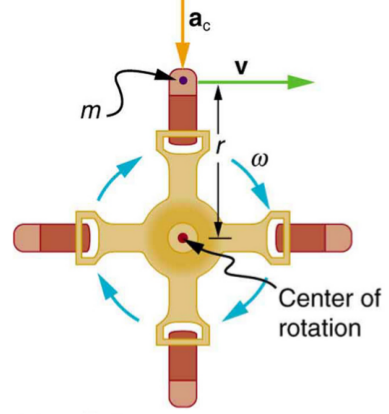
\includegraphics[width=0.25\textwidth]{cent.png}
\caption{\label{fig:cent} A blood centrifuge spinning counter-clockwise.}
\end{figure}

A diagram of a blood centrifuge is depicted in Fig. \ref{fig:cent}.  It is spinning at an angular velocity of $\omega$ and tangential velocity $v$.  In order to separate the contents in the vials (indicated with the mass $m$), the \textit{centripetal acceleration} needs to be increased by a factor of 100.  Which of the following actions will acheive this?
\begin{itemize}
\item A: Doubling the angular velocity: $\omega \rightarrow 2\omega$.
\item B: Tripling the angular velocity: $\omega \rightarrow 3\omega$.
\item C: Quadrupling the angular velocity: $\omega \rightarrow 4\omega$.
\item D: Increasing the angular velocity by a factor of 10: $\omega \rightarrow 10\omega$.
\end{itemize}
\item Suppose the radius is 8 cm, and $\omega = 2000$ revolutions per minute.  What is the centripetal acceleration? \\ \vspace{2cm}
\item Suppose the radius is 8 cm, and we measure $v = 75$ m/s.  What is $\omega$?  What is $a_C$?
\end{enumerate}

\end{document}
